\documentclass[11pt]{article}
\usepackage[margin=1in]{geometry}
\usepackage{booktabs,graphicx,float,array,longtable,caption}
\PassOptionsToPackage{hyphens}{url}\usepackage[hidelinks]{hyperref}
\usepackage{enumitem}
\usepackage{xcolor}
\setlist{nosep,leftmargin=*}
\graphicspath{{../outputs/part_a/figures/}{../outputs/part_b/figures/}}
\captionsetup{font=small,labelfont=bf}
\newcommand{\code}[1]{\texttt{#1}}
\renewcommand{\arraystretch}{1.15}

\title{\vspace{-1.5em}\textbf{AS01 Memo: Datasheet and Knowledge-Representation Experiments}\\
\large Scenario 01 --- Personalized Medication Decision Support}
\author{William Sun, Yara Yao, Xinyin Zhang, Xiuqi Zhu \\ Course: 94-864 AI Model Development}
\date{September 2026}

\begin{document}
\maketitle
\vspace{-1.5em}

\section*{Executive summary}
We are a clinical decision-support start-up piloting with chronic-disease clinics. Our model will read a patient's own account of a medication and classify the reported experience (positive / neutral / negative) so clinicians and pharmacists can see, at the point of prescribing, how similar patients tolerated a drug. We selected the UCI Drugs.com review dataset (215,063 patient reviews). Part~A shows it is large but heavily skewed: ratings are bimodal, 40\% of rows are brand/generic duplicates of the same text, and chronic conditions are only 23\% of rows. Part~B shows that generic embeddings group reviews by \emph{condition} (dense 1-NN accuracy 0.86) but not by \emph{patient experience} (all methods at or below the majority-class baseline), which is exactly the signal our tool needs. This motivates supervised fine-tuning on the rating-derived label, evaluated on macro-F1, negative-class recall, unseen-drug generalisation, and the chronic-vs-common-condition gap.

%==========================================================================
\section{Part A: Organizational scenario and dataset datasheet}

\subsection{Organizational scenario}
\textbf{Organisation.} A medical-AI start-up invited to pilot with a network of clinics treating patients with chronic conditions (hypertension, type~2 diabetes, high cholesterol, chronic pain, insomnia, depression). Patients typically take several drugs and switch between them.

\textbf{The one task.} Given a drug, the condition it is prescribed for, and a patient's free-text report, output the patient-reported experience class and the reason (e.g.\ ``NEGATIVE: gastrointestinal side effects, stopped after two weeks''). Aggregated over many reports, this gives clinicians a ``patient-voice'' summary of how a drug is tolerated by people like their patient, complementing the label and guidelines.

\textbf{Users and decisions.} Clinicians and pharmacists during prescribing and medication review. The tool ranks candidate drugs for a condition by reported tolerability and surfaces common complaints. It does not give dosing advice and does not replace clinical judgement; it is decision support only.

\textbf{Why this dataset.} It is the largest public corpus of patient-written medication experiences with a numeric outcome (rating), spanning 3,671 drugs and 916 conditions, including the chronic conditions of our pilot population.

\textbf{How this differs.} Prior work on this corpus treats it as a sentiment benchmark. We instead treat the reviews as clinician-facing tolerability evidence: the model is judged on whether it catches the harmed patients (negative-class recall) for the chronic-disease population specifically, and every row carries a Traffic Light Protocol label so that data governance is built into the pipeline rather than added afterwards.

\subsection{Dataset selection}
\begin{table}[H]\centering\small
\begin{tabular}{p{2.9cm}p{12.1cm}}\toprule
Name & Drug Review Dataset (Drugs.com), Gr\"a{\ss}er et al.\ 2018 \\
Source used & Hugging Face mirror \code{lewtun/drug-reviews} (\code{train.jsonl}, \code{test.jsonl}); also on UCI ML Repository \\
Size & 215,063 reviews (161,297 train / 53,766 test, original split); 7 original features, 11 engineered features added in Sec.~1.8 (18 in total) \\
Access / risk & Public, scraped from Drugs.com; no formal licence stated on the mirror. Per course policy an HF/UCI dataset may not be processed on CMU computing resources without approval; all work ran on a personal laptop (Apple M4 Pro). \\
Safety concerns & Reviews are patient self-reports, not clinical evidence; some contain sensitive content (see TLP labels). \\
\bottomrule\end{tabular}
\end{table}

\subsection{Feature codebook}
\begin{table}[H]\centering\small
\begin{tabular}{p{2.0cm}p{2.1cm}p{5.0cm}p{5.2cm}}\toprule
Feature & Type & Description & Utility for the scenario \\\midrule
uniqueID & integer & Row identifier assigned by the dataset authors. & None for modelling; used to trace rows across splits. \\
drugName & string, categorical (3,671 values) & Brand or generic name the reviewer chose; the same review appears under both. & Key for grouping evidence per drug; must be normalised so brand and generic are one entity. \\
condition & string, categorical (916 values) & The condition the reviewer took the drug for, as free text; 1,171 values are scraped HTML junk. & Defines the patient population; lets us evaluate the chronic-disease subgroup. \\
review & free text & The patient's written experience: effect, side effects, duration, dose, context. & The model input; carries the tolerability signal we want to surface. \\
rating & integer 1--10 & Overall satisfaction given by the reviewer. & Only outcome label available; mapped to our 3-class target. \\
date & date & Day the review was posted (2008--2017). & Drift check: drugs and vocabulary change over time. \\
usefulCount & integer & Number of readers who marked the review helpful. & Weak proxy for review quality; correlated with positivity, so not a neutral filter. \\
\bottomrule\end{tabular}
\end{table}

\subsection{Traffic Light Protocol labels}
We added \code{tlp\_label} with transparent rules (regex over review text plus a sensitive-condition list).
\begin{table}[H]\centering\small
\begin{tabular}{p{2.1cm}p{4.2cm}p{1.5cm}p{6.5cm}}\toprule
Label & Rule / meaning & Count & Example \\\midrule
TLP:CLEAR & $\le 8$ words, no first-person pronoun: generic product remark, shareable publicly. & 2,967 (1.4\%) & Topiramate / Bipolar: ``Stabilizing when used with Lamictal and Lexapro.'' \\
TLP:GREEN & Default: a patient's own experience, no extra identifiers; share within the organisation and partner clinics. & 157,803 (73.7\%) & Ibandronate / Osteoporosis: ``Taken one dose so far and do not believe that I will take no more \ldots severe pains in my stomach.'' \\
TLP:AMBER & Mentions third parties (my son, my wife), explicit age, pregnancy, or a named doctor; de-identify before use. & 43,076 (20.1\%) & Phentermine / Weight Loss: ``I am 56 years old, female weighed in today at 160 \ldots'' \\
TLP:RED & Crisis or highly sensitive content (suicidal ideation, overdose, HIV, abuse, substance dependence) or a sensitive condition; excluded from training by default. & 10,232 (4.8\%) & Aripiprazole / Schizophrenia: ``No voices, no visual hallucinations. I still struggle with mild paranoia \ldots'' \\
\bottomrule\end{tabular}
\end{table}

\subsection{Descriptive statistics and data profiling}
\begin{table}[H]\centering\small
\caption{Feature profile (raw data, $n=215{,}063$).}
\begin{tabular}{lrrrr}\toprule
Feature & dtype & missing & missing \% & unique \\\midrule
uniqueID & int & 0 & 0 & 215,063 \\
drugName & str & 0 & 0 & 3,671 \\
condition & str & 1,194 & 0.56 & 916 \\
review & str & 0 & 0 & 128,478 \\
rating & int & 0 & 0 & 10 \\
date & date & 0 & 0 & 3,579 \\
usefulCount & int & 0 & 0 & 397 \\
\bottomrule\end{tabular}
\end{table}

\begin{table}[H]\centering\small
\caption{Numeric features, raw and engineered (after cleaning, $n=214{,}078$).}
\footnotesize\begin{tabular}{lrrrrrrrrrr}\toprule
Feature & min & max & mean & median & std & Q1 & Q3 & range & skew & kurt. \\\midrule
rating & 1 & 10 & 6.98 & 8 & 3.28 & 5 & 10 & 9 & $-0.79$ & $-0.90$ \\
usefulCount & 0 & 1,291 & 28.1 & 16 & 36.4 & 6 & 36 & 1,291 & 4.49 & 56.7 \\
review\_word\_len & 3 & 1,894 & 85.0 & 85 & 44.6 & 49 & 126 & 1,891 & 0.94 & 23.0 \\
review\_char\_len & 8 & 10,431 & 449 & 446 & 234 & 257 & 676 & 10,423 & 1.02 & 26.5 \\
review\_sentence\_count & 1 & 91 & 5.95 & 6 & 3.33 & 3 & 8 & 90 & 0.97 & 6.95 \\
drug\_review\_count & 1 & 4,920 & 833 & 438 & 1,115 & 129 & 1,072 & 4,919 & 2.24 & 4.63 \\
review\_year & 2008 & 2017 & 2014.0 & 2015 & 2.71 & 2012 & 2016 & 9 & $-0.70$ & $-0.76$ \\
\bottomrule\end{tabular}
\end{table}

\begin{table}[H]\centering\small
\caption{Categorical / text features: class distribution and long tail.}
\footnotesize\begin{tabular}{lrrrrr}\toprule
Feature & unique & top-1 share & top-10 share & values with $\le 5$ rows & values with 1 row \\\midrule
drugName & 3,671 & 2.3\% (Levonorgestrel) & 13.3\% & 1,783 & 798 \\
condition & 916 & 18.0\% (Birth Control) & 46.2\% & 341 & 113 \\
\midrule
rating (\%) & \multicolumn{5}{l}{1: 13.5 \; 2: 4.3 \; 3: 4.1 \; 4: 3.1 \; 5: 5.0 \; 6: 3.9 \; 7: 5.8 \; 8: 11.7 \; 9: 17.1 \; 10: 31.6} \\
sentiment\_label & \multicolumn{5}{l}{POSITIVE 66.1\% \; NEGATIVE 25.0\% \; NEUTRAL 8.9\%} \\
tlp\_label & \multicolumn{5}{l}{GREEN 73.7\% \; AMBER 20.1\% \; RED 4.8\% \; CLEAR 1.4\%} \\
is\_chronic\_condition & \multicolumn{5}{l}{1: 22.7\% \; 0: 77.3\%} \\
side\_effect\_flag & \multicolumn{5}{l}{1: 55.1\% \; 0: 44.9\%} \\
\bottomrule\end{tabular}
\end{table}

\textbf{Data quality.} Every review is wrapped in literal quotes and 65\% contain HTML entities (fixed by unescaping). 1,171 \code{condition} values are the scraped string ``\ldots\code{</span>} users found this comment helpful'' (set to missing). Most importantly, 86,068 distinct review texts appear more than once and 86,049 of them are the same review listed under a brand and a generic drug name: 40\% of the rows are duplicates at the text level. Exact duplicates (83) and reviews under three words were dropped, leaving 214,078 rows.

\begin{figure}[H]\centering
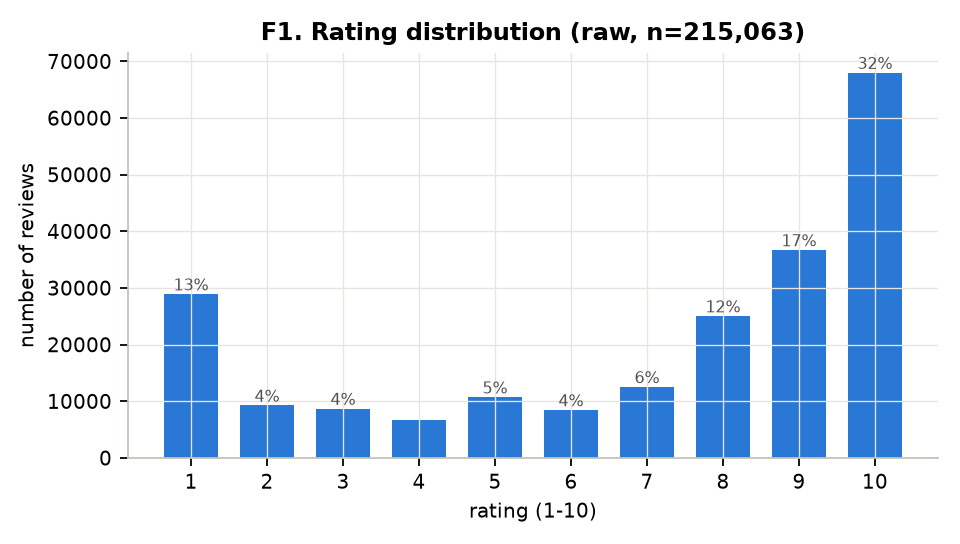
\includegraphics[width=.49\textwidth]{F1_rating_hist}\hfill
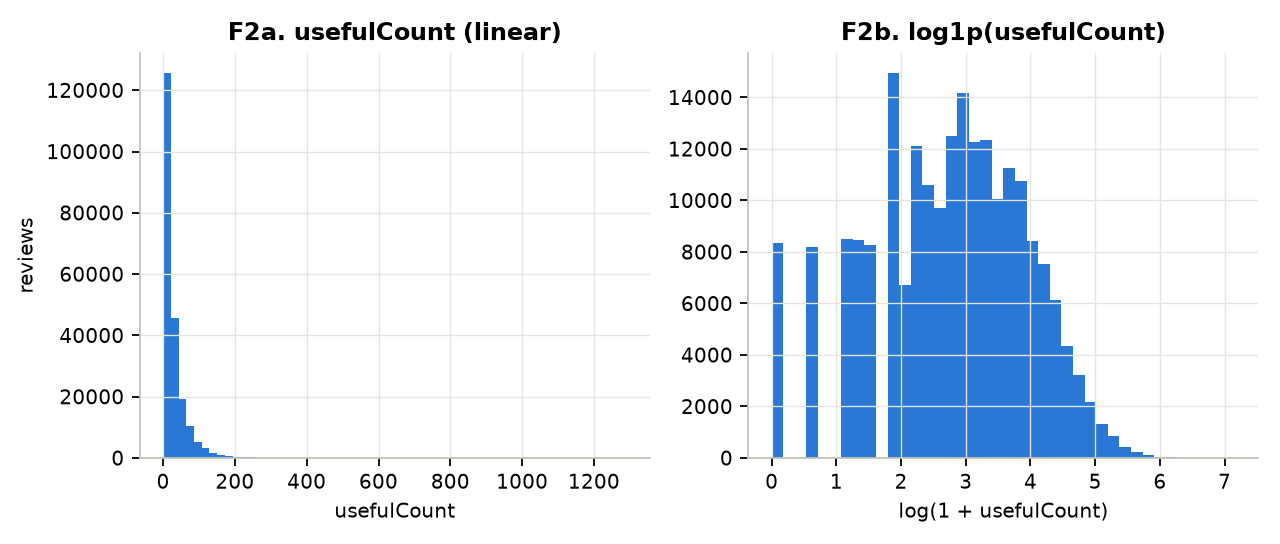
\includegraphics[width=.49\textwidth]{F2_usefulcount_hist}\\[2pt]
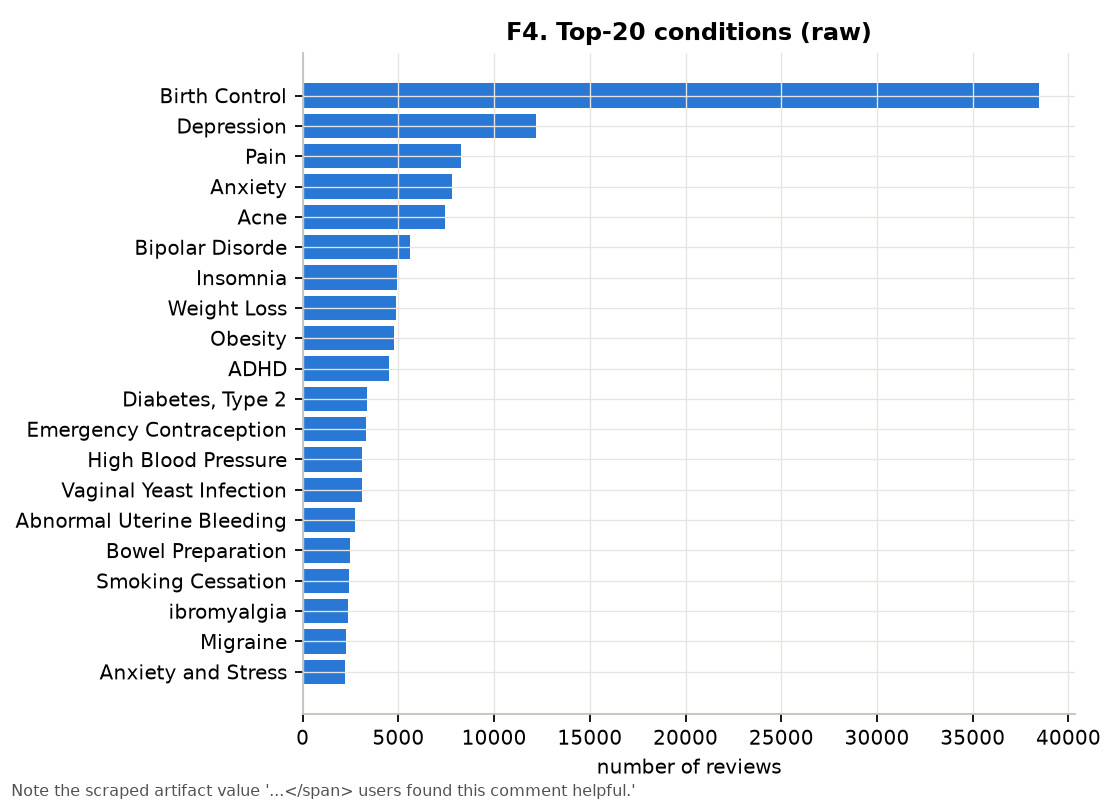
\includegraphics[width=.49\textwidth]{F4_top_conditions}\hfill
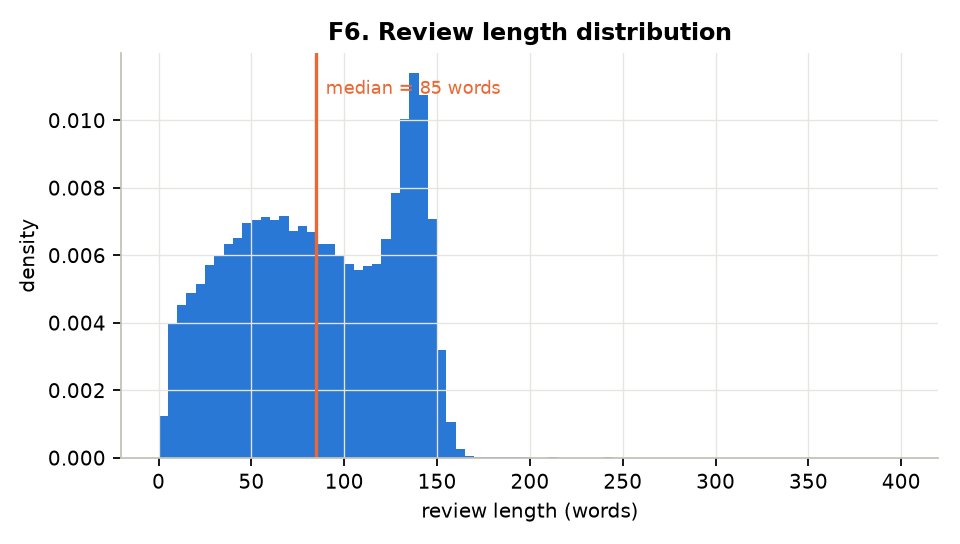
\includegraphics[width=.49\textwidth]{F6_review_length_density}
\caption{Rating histogram (bimodal), usefulCount on linear and log scale, top-20 conditions, and review length density.}
\end{figure}

\begin{figure}[H]\centering
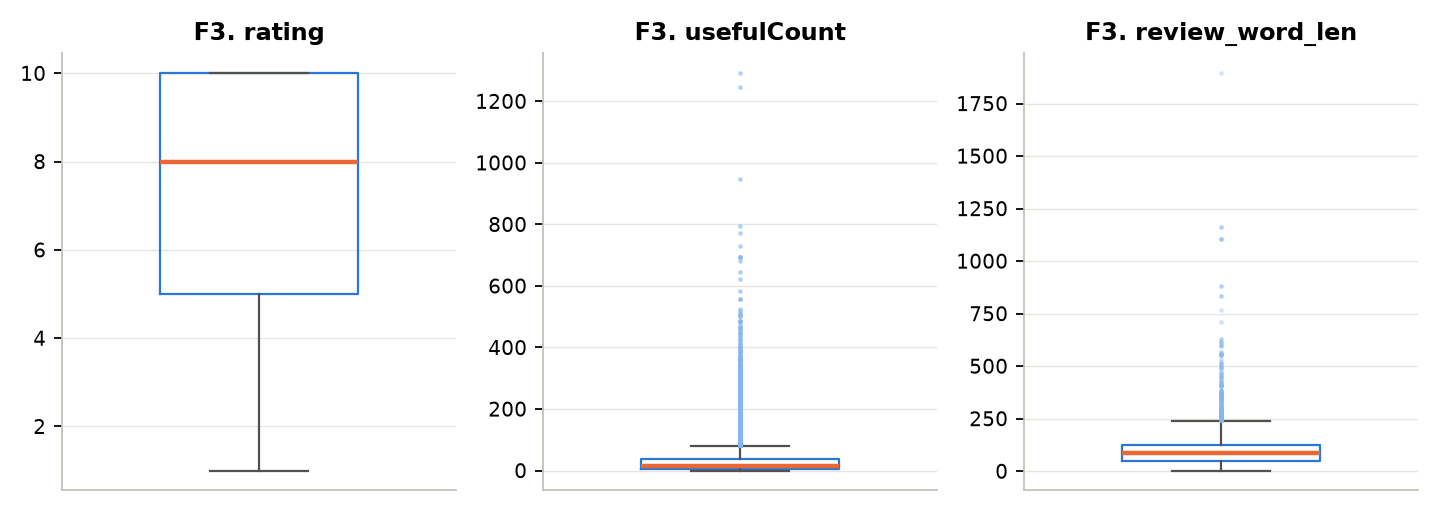
\includegraphics[width=.49\textwidth]{F3_boxplots}\hfill
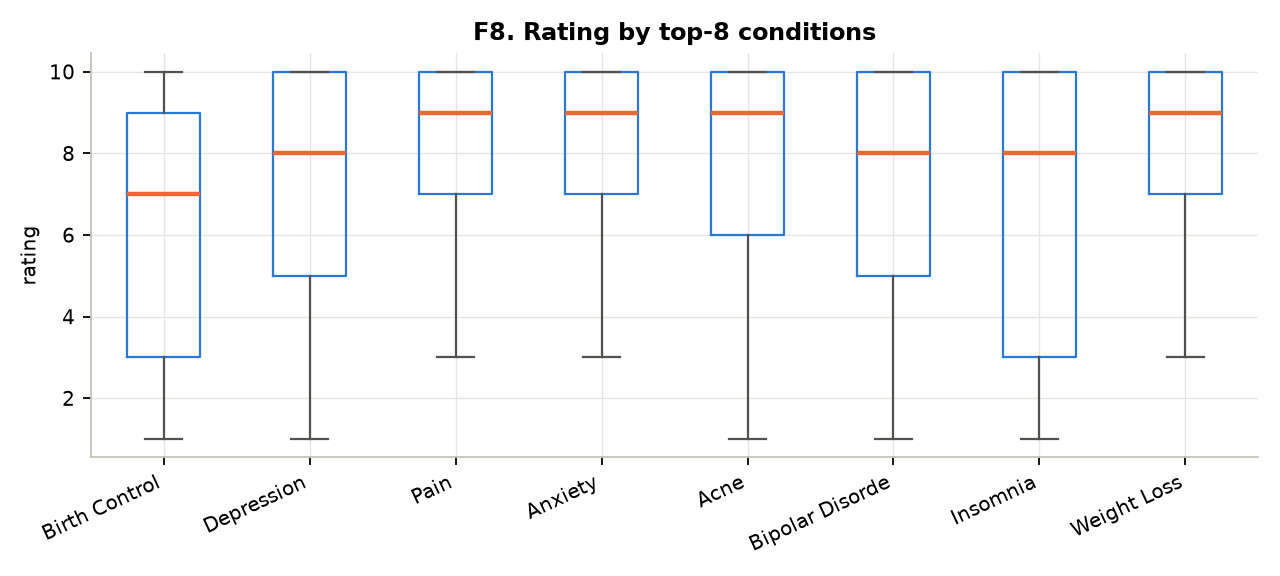
\includegraphics[width=.49\textwidth]{F8_rating_by_condition}
\caption{Boxplots of the numeric features and rating by the eight most frequent conditions.}
\end{figure}

\subsection{Normal vs.\ non-normal distributions}
\begin{table}[H]\centering\small
\caption{Normality evidence (Shapiro--Wilk on a 5,000-row sample; D'Agostino $K^2$ on all rows).}
\footnotesize\begin{tabular}{lrrrrl}\toprule
Feature & skew & exc.\ kurt. & Shapiro $W$ & $W$, $\log(1+x)$ & verdict \\\midrule
rating & $-0.79$ & $-0.90$ & 0.803 & 0.732 & non-normal, bimodal \\
usefulCount & 4.49 & 56.7 & 0.642 & 0.984 & non-normal, $\approx$ log-normal \\
review\_word\_len & 0.94 & 23.0 & 0.950 & 0.877 & non-normal, right-skewed \\
review\_sentence\_count & 0.97 & 6.95 & 0.962 & 0.952 & non-normal, right-skewed \\
drug\_review\_count & 2.24 & 4.63 & 0.697 & 0.967 & non-normal, long tail \\
\bottomrule\end{tabular}
\end{table}
\begin{figure}[H]\centering
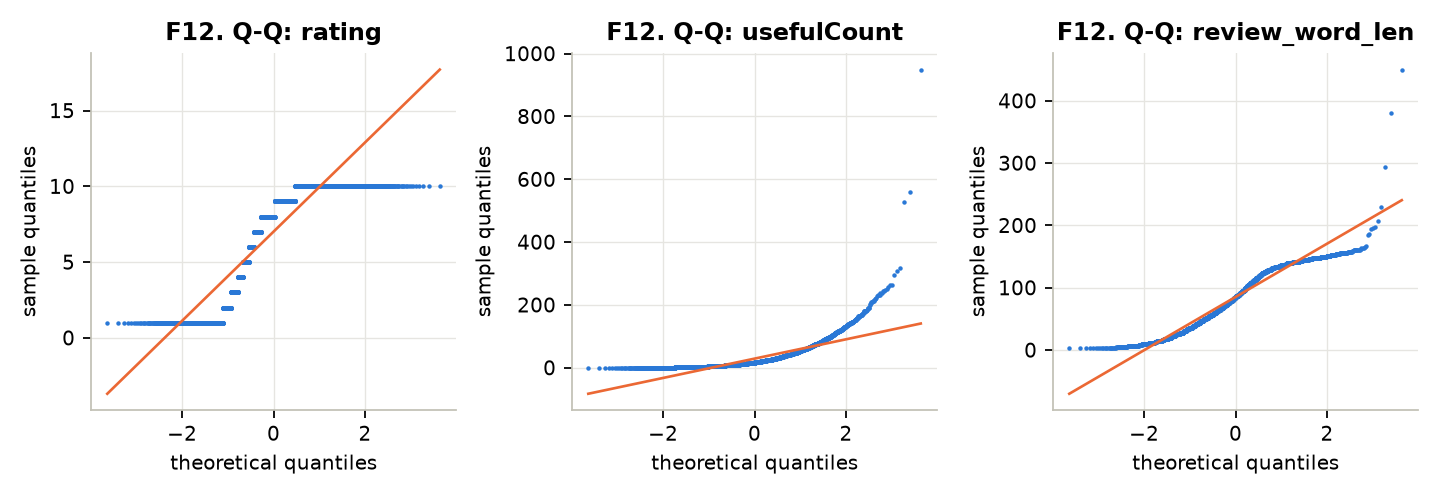
\includegraphics[width=.95\textwidth]{F12_qq_plots}
\caption{Q--Q plots against a normal distribution: the staircase (rating), the exploding upper tail (usefulCount) and the bent tails (review length) all reject normality.}
\end{figure}

None of the features is normally distributed (all tests $p<10^{-30}$). \emph{rating} is the clearest case: a third of reviews are 10 and 13\% are 1, so it is bimodal with a hollow middle, and the mean (6.98) sits below the median (8). \emph{usefulCount} is a count with a long right tail (median 16, max 1,291, kurtosis 57); after a log transform it is close to normal, so it is approximately log-normal. \emph{Review length} is right-skewed but not log-normal: most reviews are 50--130 words with a thin tail up to 1,900. The categorical features are long-tailed: ten conditions cover 46\% of rows, and half of all drugs have six or fewer reviews.

\subsection{Impact of the distributions on model development}
The skew in \emph{rating} is the main risk. Mapped to three classes it gives 66\% positive, 25\% negative and 9\% neutral, so a model trained on it directly will default to ``positive'' and under-report the negative experiences a safety tool exists to surface; the hollow middle of the bimodal scale also makes neutral the smallest and most ambiguous class. We therefore balance the training set and judge the model on macro-F1 and negative-class recall rather than accuracy. The long tails matter for whom the model serves: 1,783 drugs have five or fewer reviews, chronic conditions are 23\% of rows while Birth Control alone is 18\%, so aggregate metrics would describe contraceptive users rather than our pilot population and generalisation to rarely reviewed drugs is uncertain; we evaluate per condition and hold out unseen drugs. Two further properties shape preprocessing: the brand/generic duplication would leak 40\% of test texts into training unless rows are de-duplicated before splitting, and \emph{usefulCount}'s heavy tail and positive correlation with rating (Spearman 0.28) rule it out as a neutral quality weight.

\subsection{Feature engineering}
\begin{table}[H]\centering\small
\begin{tabular}{p{2.8cm}p{1.9cm}p{4.3cm}p{1.5cm}p{3.9cm}}\toprule
New feature & Source & How created & Type & Why useful \\\midrule
sentiment\_label & rating & 1--4 NEGATIVE, 5--6 NEUTRAL, 7--10 POSITIVE & categorical & The SFT target: patient-reported experience class. \\
side\_effect\_flag & review & regex over 20 common side-effect terms (nausea, dizziness, weight gain, \ldots) & binary & Flags reviews carrying safety content the tool must surface. \\
is\_chronic\_condition & condition & membership in a curated list of 32 chronic conditions & binary & Identifies the pilot population for subgroup evaluation. \\
tlp\_label & review, condition & rule-based Traffic Light Protocol (Sec.~1.4) & categorical & Data-protection filter before training. \\
review\_word\_len, review\_sentence\_count & review & token and sentence-boundary counts after HTML unescape & integer & Chunking and sequence-length decisions; proxy for information content. \\
drug\_review\_count & drugName & group size & integer & Exposure of each drug in training data (long-tail risk). \\
condition\_clean, review\_year & condition, date & junk values set to missing; year component & string, integer & Removes fake classes; drift analysis. \\
\bottomrule\end{tabular}
\end{table}

\begin{table}[H]\centering\small
\caption{Evaluation of engineered features against the original rating.}
\begin{tabular}{lrrrr}\toprule
Group & $n$ & mean rating & median & \% POSITIVE \\\midrule
side\_effect\_flag = 0 & 96,148 & 7.11 & 9 & 67.8 \\
side\_effect\_flag = 1 & 117,930 & 6.89 & 8 & 64.7 \\
is\_chronic = 0 & 165,581 & 6.94 & 8 & -- \\
is\_chronic = 1 & 48,497 & 7.14 & 8 & -- \\
\midrule
\multicolumn{5}{l}{Spearman: rating--usefulCount 0.28; rating--word\_len 0.01;} \\
\multicolumn{5}{l}{word\_len--side\_effect\_flag 0.26; word\_len--sentence\_count 0.81} \\
\bottomrule\end{tabular}
\end{table}

\textbf{Assessment.} \code{sentiment\_label} turns a bimodal 10-point scale into three well-separated groups (mean rating 1.9 / 5.4 / 9.1) and is the only feature that operationalises the project objective. \code{side\_effect\_flag} adds information the rating does not carry (55\% of reviews mention a side effect, and reviews with the flag are longer), but it barely separates satisfaction: patients report side effects even when satisfied, so the keyword alone cannot replace reading the text. \code{is\_chronic\_condition} shows the pilot population rates drugs slightly higher than average, so overall metrics would mask their errors. \code{tlp\_label} reduces governance ambiguity by making the sharing status of each row explicit. Length features are redundant with each other (0.81) but uncorrelated with rating, so they inform preprocessing rather than prediction.

%==========================================================================
\section{Part B: Tokenization and embedding experiments}
\textbf{Sample.} 800 de-duplicated reviews of 20--220 words, 100 each from four high-frequency conditions (Birth Control, Depression, Pain, Acne) and four chronic conditions (Diabetes Type~2, High Blood Pressure, High Cholesterol, Insomnia); seed 42. Sentiment mix 476 / 92 / 232 (POS / NEU / NEG).

\subsection{Choices and rationale}
\textbf{Tokenizer.} The starter word tokenizer (lower-case, strip punctuation) is our primary strategy because it is fully inspectable and patient reviews are short, informal text. We added two contrasts: the same tokenizer with stopwords removed, and 40-word fixed chunks with mean pooling, to test whether chunking helps or hurts. We also report the dense model's WordPiece subword tokenizer to show how a general-domain vocabulary handles drug names.

\textbf{Embeddings.} Bag-of-Words and TF-IDF (starter, sparse) are the transparent baselines. For a dense model we used \code{all-MiniLM-L6-v2} (384-d, sentence-transformers): EmbeddingGemma is gated on Hugging Face and required licence approval we did not yet have; the script accepts it as a drop-in replacement.

\textbf{Similarity.} Cosine similarity for both sparse and dense vectors, because it is length-invariant (reviews vary from 20 to 220 words) and is the metric the dense model was trained with.

\textbf{Evaluation.} For each review we find its nearest neighbour (leave-one-out) and ask whether it shares the condition and whether it shares the sentiment label; chance is 0.125 for condition and the majority-class baseline is 0.595 for sentiment. We also compare within- and between-condition similarity (Cohen's $d$).

\subsection{Results}
Table~\ref{tab:eval} summarises the experiment; the full results (tokenization statistics, subword splits, per-condition accuracy, similarity distributions, condition heatmaps, query retrieval and most/least similar pairs) are in Appendix~B as required.

\begin{table}[H]\centering\small
\caption{Leave-one-out nearest-neighbour evaluation and similarity separation (cosine).}\label{tab:eval}
\begin{tabular}{lrrrrrrr}\toprule
Method & cond.\ 1-NN & cond.\ 5-NN & sent.\ 1-NN & within & between & gap & $d$ \\\midrule
BoW & 0.385 & 0.438 & 0.500 & 0.382 & 0.358 & 0.024 & 0.18 \\
BoW, no stopwords & 0.630 & 0.725 & 0.536 & 0.103 & 0.056 & 0.047 & 0.75 \\
TF-IDF & 0.648 & 0.743 & 0.569 & 0.120 & 0.096 & 0.025 & 0.48 \\
TF-IDF, no stopwords & 0.719 & 0.808 & 0.564 & 0.056 & 0.027 & 0.029 & 0.78 \\
Dense (MiniLM) & \textbf{0.859} & \textbf{0.889} & 0.571 & 0.467 & 0.321 & 0.147 & \textbf{1.29} \\
Dense, chunked & 0.801 & 0.841 & 0.578 & 0.496 & 0.366 & 0.130 & 1.07 \\
\midrule
chance / majority & 0.125 & 0.125 & 0.595 & & & & \\
\bottomrule\end{tabular}
\end{table}

\textbf{Qualitative checks.} BoW's most similar pair joins a Pain review to a High Cholesterol review because both are long and share function words; dense's most similar pair (0.88) is two statin users describing muscle and joint pain. For the query ``dizziness and fatigue after starting blood pressure medication'', TF-IDF returns reviews that merely repeat ``blood pressure'', while dense returns a clonidine review that literally describes dizzy spells and fatigue (Appendix Table~\ref{tab:query}; most and least similar pairs in Table~\ref{tab:pairs}).

\subsection{Interpretation and implications}
\textbf{Model performance and generalisation.} Representation quality matters more than tokenization detail: the dense model finds a same-condition neighbour 86\% of the time against 65\% for TF-IDF, with a within/between separation of $d=1.29$ versus $0.48$. Cheap preprocessing still pays off for sparse methods, since removing stopwords (half of all tokens) lifts BoW from 0.39 to 0.63, whereas chunking hurts (0.86 $\to$ 0.80) because reviews are short enough to embed whole. The dense model gains most on exactly the chronic conditions where TF-IDF is weakest (High Blood Pressure 0.43 $\to$ 0.83), because it matches paraphrases such as ``bp'', ``pressure'' and ``150/90'' rather than exact terms. The subword splits show the limit of that transfer: the pretrained tokenizer has no unit for metformin or lisinopril, so drug identity is reconstructed from fragments and a domain-adapted vocabulary or fine-tuning remains necessary.

\textbf{Bias and representation of concepts.} No representation separates patient experience: every sentiment 1-NN rate is at or below the 0.595 majority baseline and $d\approx 0$. Off-the-shelf embeddings encode what a review is about, not how the patient fared, so a retrieval-only system would hand clinicians topically matched but experientially mixed evidence, and the heatmap shows it would also blur Depression, Insomnia and hypertension reviews through their shared symptom vocabulary.

\textbf{Dataset quality and future decisions.} The brand/generic duplication had to be removed before this experiment or 1-NN accuracy is trivially inflated by identical texts; stopword share (49\%), HTML entities and scraped condition strings degrade sparse representations more than dense ones. For the project this means: fine-tune on the rating-derived label, since the experience signal is absent from generic embeddings; embed whole reviews within a 512-token limit without chunking; prefer a model whose tokenizer, or an added vocabulary, covers drug names; evaluate per condition with the chronic subgroup reported separately; and de-duplicate by text before every split.

%==========================================================================
\section{Part C: Research plan and analysis memo}
\subsection{Research questions}
\begin{enumerate}
\item[\textbf{RQ1}] Does a small open LLM fine-tuned on patient reviews classify patient-reported medication experience better than its zero-shot version and a TF-IDF baseline, and how much does performance drop on drugs never seen in training?
\item[\textbf{RQ2}] Which knowledge representation (sparse lexical, generic dense, fine-tuned) best captures patient \emph{experience} rather than \emph{topic}, and does that translate into higher negative-class recall?
\item[\textbf{RQ3}] How do the skewed rating distribution and the over-representation of non-chronic conditions bias the fine-tuned model against the chronic-disease population, and does class balancing reduce the gap?
\end{enumerate}

\subsection{Plan}
\begin{table}[H]\centering\small
\begin{tabular}{p{2.8cm}p{12.2cm}}\toprule
Model & Llama~3.2~1B/3B-Instruct or Qwen2.5-1.5B-Instruct, LoRA ($r=16$), 2 epochs, lr $2\times10^{-4}$, 512 tokens, assistant-only loss; laptop (MLX) or free Colab GPU. \\
Data & \code{data/sft/}: TLP:RED removed; brand/generic de-duplicated (214,078 $\to$ 121,012 rows); 10\% of drugs (305) held out entirely; stratified 80/10/10 of the rest; training set capped at 8,000 per class (23,752 rows), evaluation splits keep the natural 66/25/9 mix. \\
Baselines & zero-shot and 5-shot base model; TF-IDF + logistic regression. \\
Metrics & macro-F1 (primary); NEGATIVE recall $\ge 0.85$ (safety); macro-F1 drop on unseen drugs $\le 0.05$ (RQ1); chronic vs high-frequency F1 gap $\le 0.10$ (RQ3); error analysis of 50 misclassified reviews. \\
Timeline & Wk 1--2 baselines and first LoRA run (AS02); Wk 3--4 balanced vs unbalanced ablation, unseen-drug test; Wk 5 error analysis and subgroup report; Wk 6--7 report and poster. \\
Data protection & TLP filter applied before training; AMBER rows scheduled for automated de-identification (age, relatives, named clinicians) in future work; outputs never expose review text to end users, only aggregates. \\
\bottomrule\end{tabular}
\end{table}

\subsection{Analysis memo}
Part~A and Part~B together tell one story. The dataset is large and relevant but not ready: its outcome variable is bimodal and imbalanced, its entities are duplicated across brand and generic names, and its population is dominated by contraceptive users rather than the chronic-disease patients in our pilot. Part~B then shows that the representation problem is not topical: even a hand-rolled TF-IDF finds the condition of a review two thirds of the time and a small dense model does so 86\% of the time, but neither can tell a satisfied patient from a harmed one. That is precisely the distinction a medication-safety tool must make, so retrieval over generic embeddings would present clinicians with topically relevant but experientially mixed evidence. The implication for the project is clear: supervise the model on the experience label, balance the training data, hold out drugs to test generalisation, and report the chronic subgroup separately. Success is not accuracy but negative-class recall on the patients who were harmed, and the plan above is designed to produce that evidence for the innovation board within the seven-week window.

%==========================================================================
\section*{References}
\begin{enumerate}[label={[\arabic*]}]
\item Gr\"a{\ss}er, F., Kallumadi, S., Malberg, H., Zaunseder, S. (2018). Aspect-based sentiment analysis of drug reviews applying cross-domain and cross-data learning. \emph{Proc.\ 2018 Int.\ Conf.\ on Digital Health}, 121--125.
\item UCI Machine Learning Repository. Drug Review Dataset (Drugs.com). \url{https://archive.ics.uci.edu/dataset/462}
\item Hugging Face dataset mirror \code{lewtun/drug-reviews}. \url{https://huggingface.co/datasets/lewtun/drug-reviews}
\item Gebru, T. et al. (2021). Datasheets for datasets. \emph{Communications of the ACM}, 64(12), 86--92.
\item CISA. Traffic Light Protocol (TLP) definitions and usage. \url{https://www.cisa.gov/news-events/news/traffic-light-protocol-tlp-definitions-and-usage}
\item Reimers, N., Gurevych, I. (2019). Sentence-BERT. \emph{EMNLP}. Model: \code{all-MiniLM-L6-v2} (sentence-transformers).
\item Hu, E. et al. (2022). LoRA: Low-rank adaptation of large language models. \emph{ICLR}.
\item Course starter kit \code{as01\_v02} (tokenizers, BoW/TF-IDF, cosine similarity, EmbeddingGemma helpers).
\item Software: Python 3.13; pandas 3.0; NumPy 2.5; SciPy 1.18; Matplotlib 3.11; sentence-transformers 6.0; PyTorch 2.14; Hugging Face \code{datasets-server} API.
\end{enumerate}

%==========================================================================
\appendix
\section{Part A: additional figures}
\begin{figure}[H]\centering
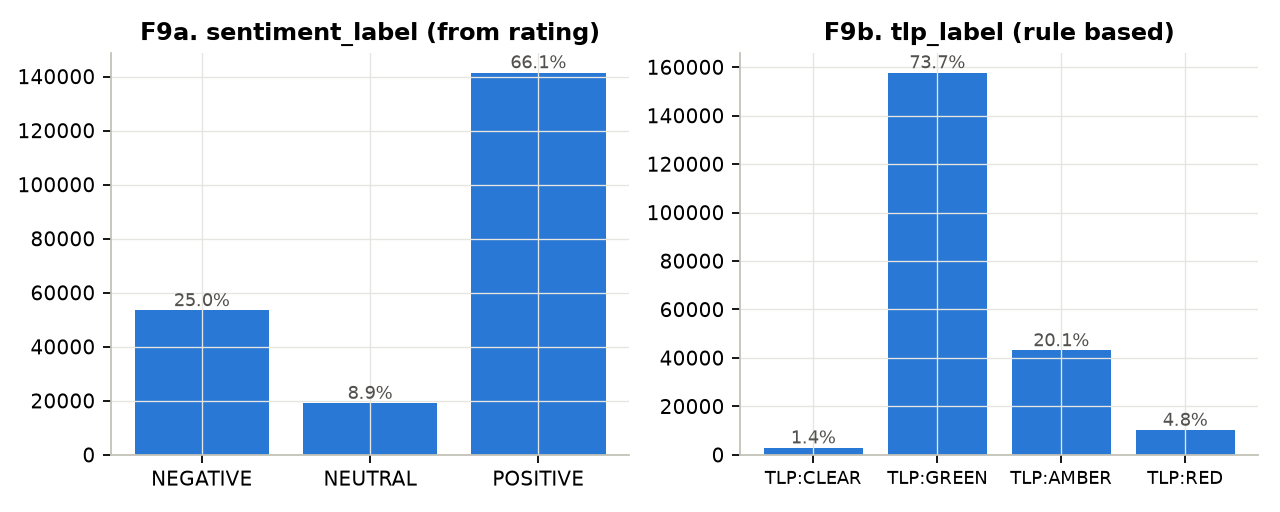
\includegraphics[width=.49\textwidth]{F9_engineered_labels}\hfill
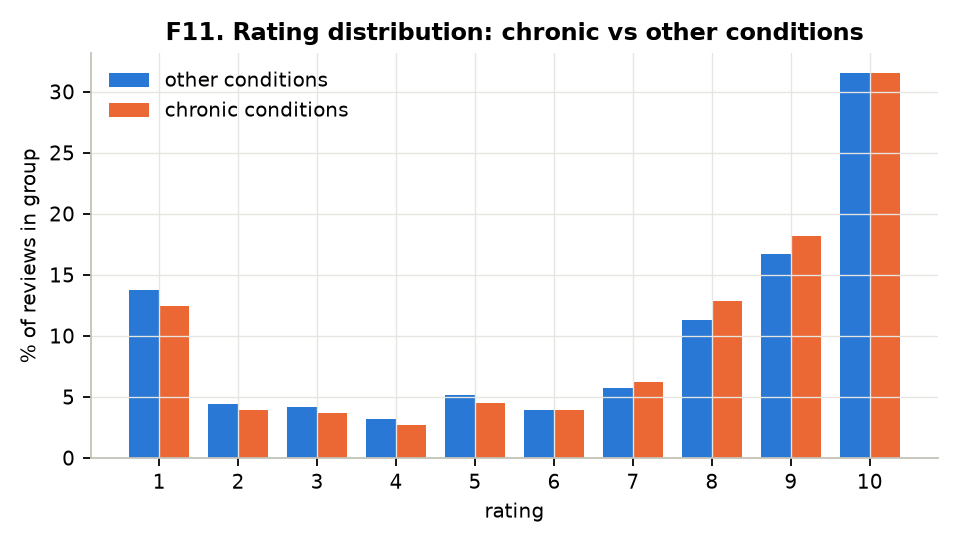
\includegraphics[width=.49\textwidth]{F11_rating_chronic_vs_other}\\[2pt]
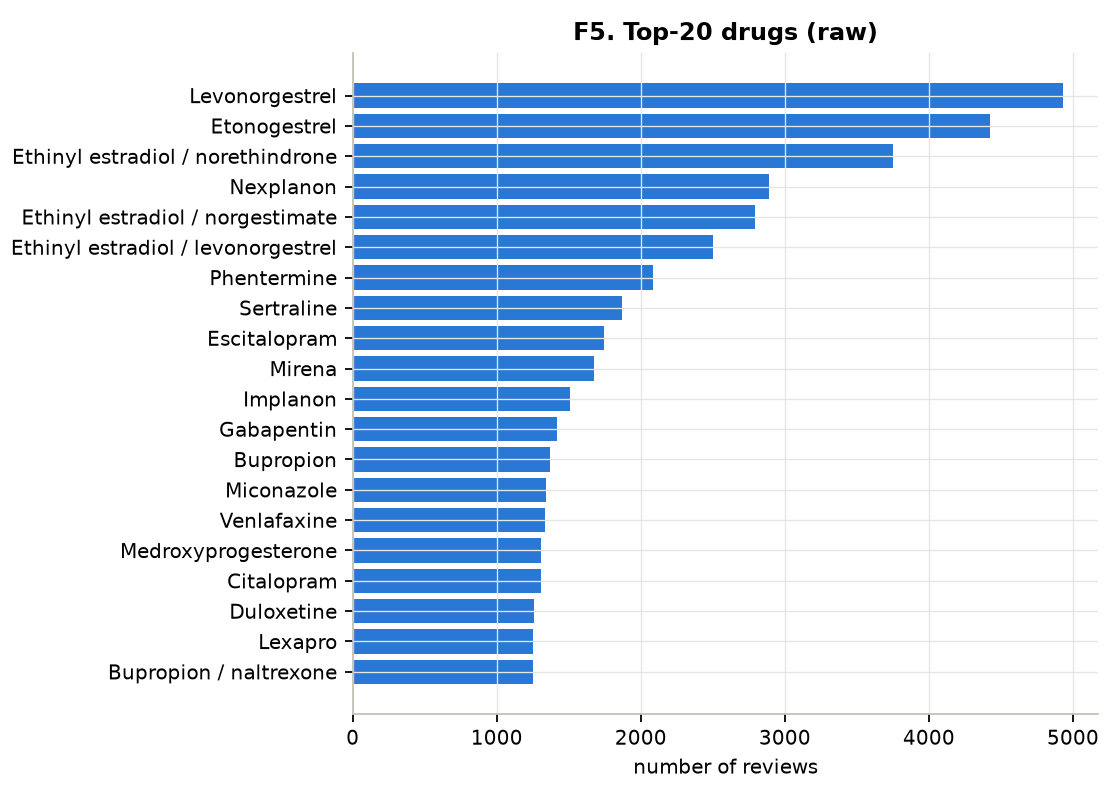
\includegraphics[width=.49\textwidth]{F5_top_drugs}\hfill
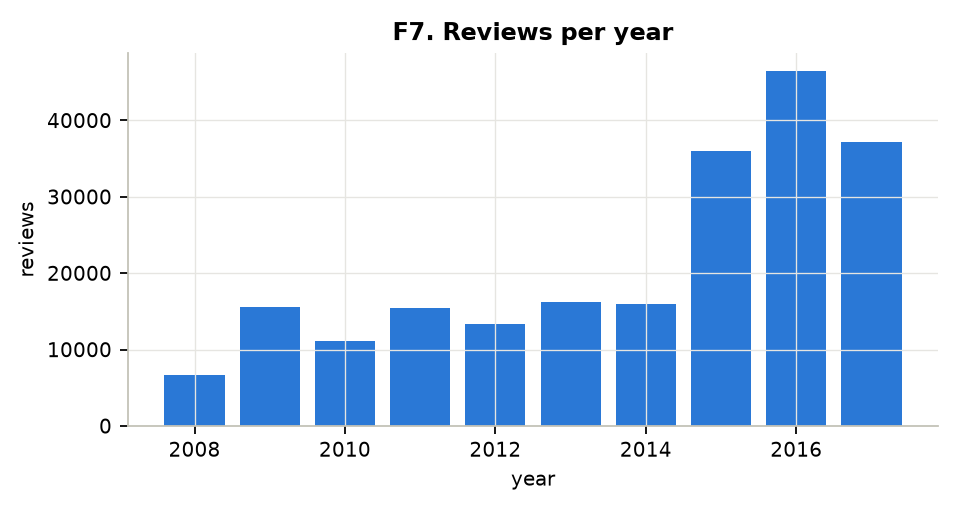
\includegraphics[width=.49\textwidth]{F7_reviews_per_year}
\caption{Engineered label distributions; rating by chronic flag; top-20 drugs; reviews per year.}
\end{figure}

\section{Part B: experimental results}
\begin{table}[H]\centering\small
\caption{Tokenization statistics and subword splits of chronic-disease drug names.}
\begin{tabular}{lrrr}\toprule
Strategy & units / review (mean) & median & vocabulary \\\midrule
word & 85.9 & 83 & 5,092 \\
word, no stopwords & 42.8 & 42 & 4,945 \\
WordPiece (MiniLM) & 108.0 & 103.5 & 4,996 \\
fixed chunk (40 words) & 2.6 chunks & 3 & -- \\
\bottomrule\end{tabular}\quad
\begin{tabular}{ll}\toprule
Drug & WordPiece pieces \\\midrule
metformin & met \#\#form \#\#in (3) \\
lisinopril & li \#\#sin \#\#op \#\#ril (4) \\
atorvastatin & at \#\#or \#\#vas \#\#tat \#\#in (5) \\
hydrochlorothiazide & 7 pieces \\
insulin & insulin (1) \\
\bottomrule\end{tabular}
\end{table}

\begin{figure}[H]\centering
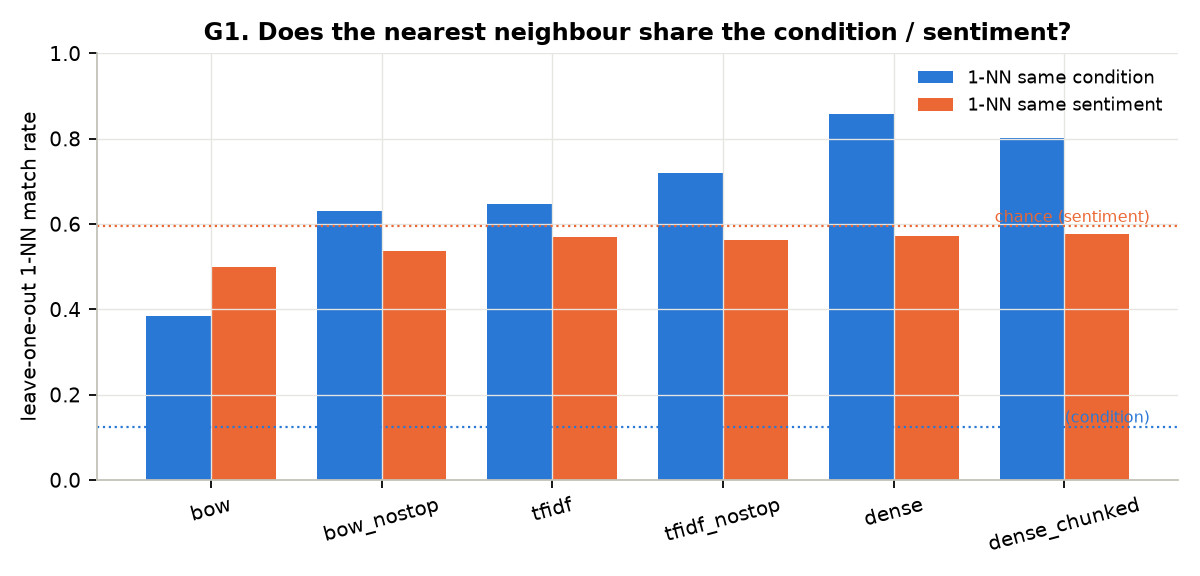
\includegraphics[width=.55\textwidth]{G1_nn_match_rates}\hfill
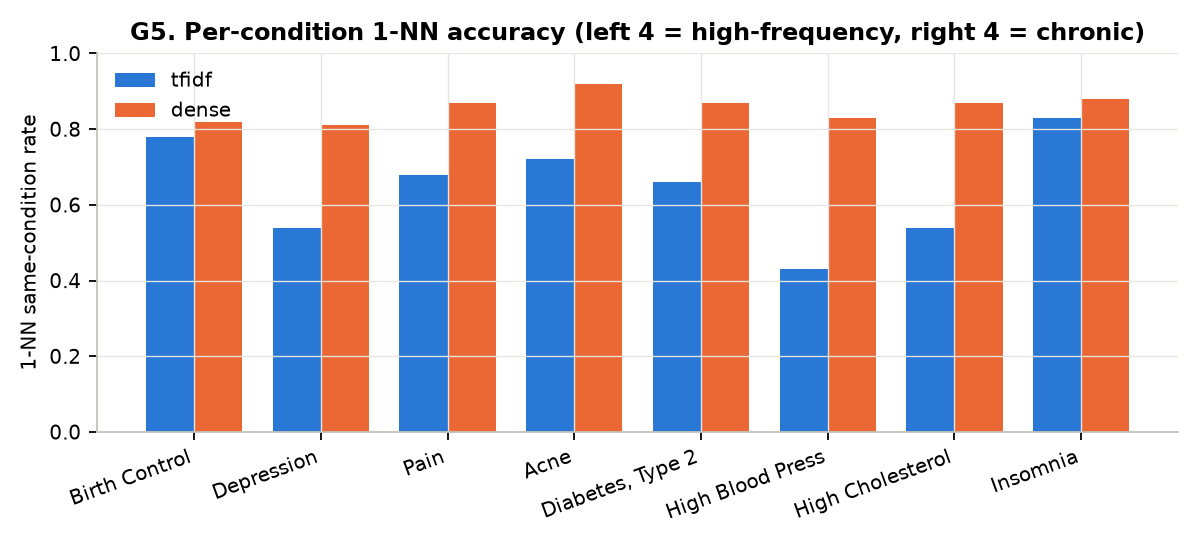
\includegraphics[width=.44\textwidth]{G5_per_condition_nn}
\caption{Left: 1-NN match rates. Right: per-condition accuracy; dense embeddings close the gap on the chronic conditions where TF-IDF is weakest (High Blood Pressure 0.43 $\to$ 0.83, High Cholesterol 0.54 $\to$ 0.87).}
\end{figure}
\begin{figure}[H]\centering
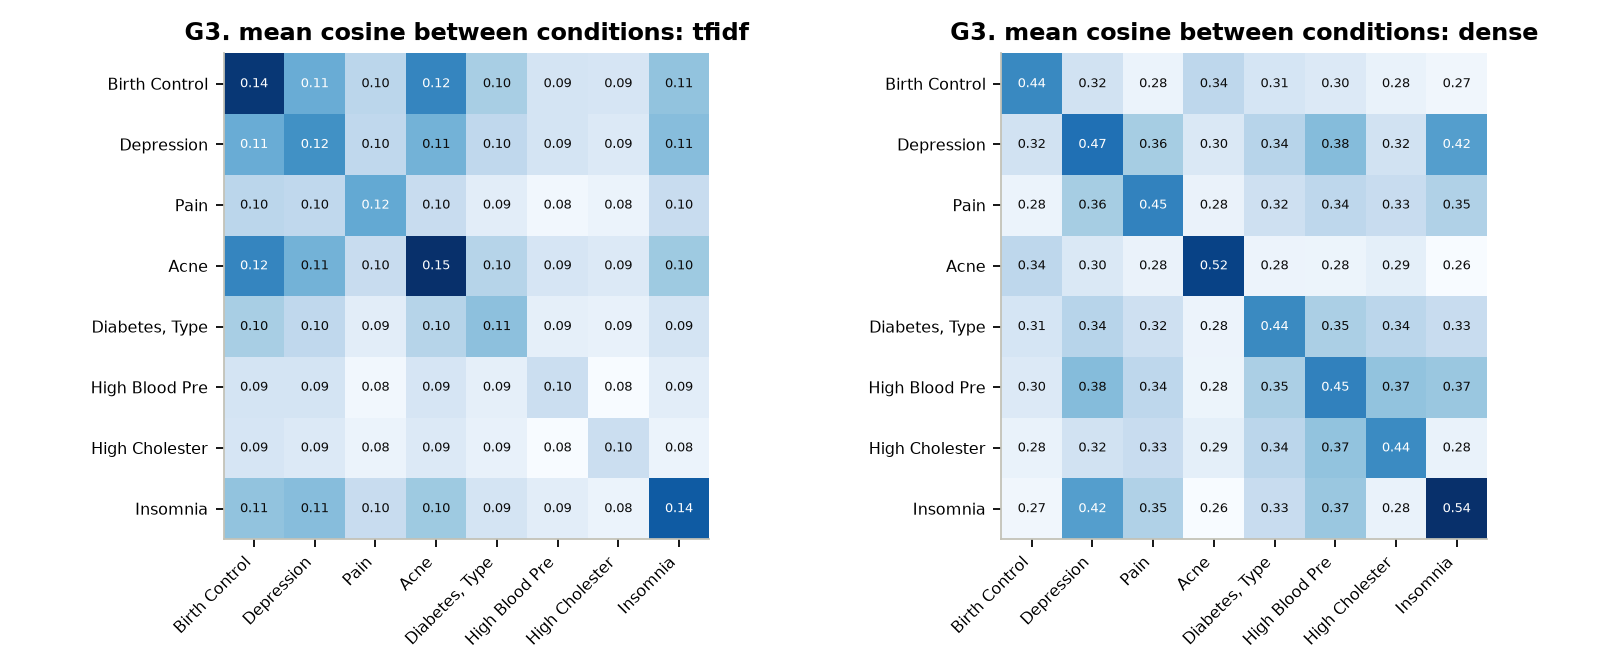
\includegraphics[width=.95\textwidth]{G3_condition_heatmaps}
\caption{Mean cosine between conditions. Dense embeddings place Depression next to Insomnia (0.42) and High Blood Pressure (0.38): symptom overlap (sleep, fatigue) that is clinically meaningful but also a source of confusion.}
\end{figure}

\begin{figure}[H]\centering
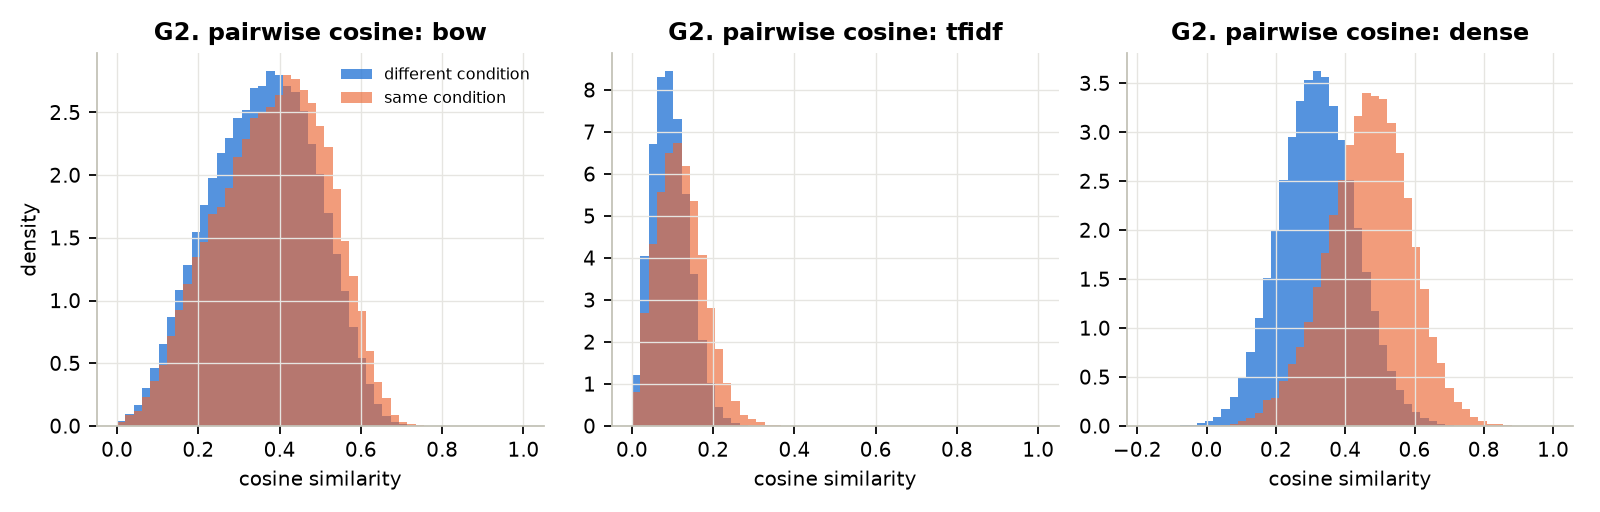
\includegraphics[width=.95\textwidth]{G2_similarity_distributions}
\caption{Pairwise cosine similarity for same-condition vs different-condition pairs: only the dense model separates the two distributions.}
\end{figure}

\begin{table}[H]\centering\small
\caption{Top TF-IDF terms per condition (word tokenizer, stopwords kept): function words dominate, which explains the weak BoW/TF-IDF separation.}
\begin{tabular}{ll}\toprule
Birth Control & i, the, and, my, it, was, a, to, \textbf{period}, have, \textbf{pill} \\
Depression & i, and, to, the, it, \textbf{depression}, was, a, my, for, of, \textbf{anxiety} \\
High Blood Pressure & i, \textbf{pressure}, my, and, the, to, \textbf{blood}, it, a, \textbf{bp} \\
Insomnia & i, \textbf{sleep}, it, and, to, \textbf{night}, the, a, \textbf{ambien} \\
\bottomrule\end{tabular}
\end{table}

\begin{table}[H]\centering\small
\caption{Clinical query retrieval, top-1 result per method.}\label{tab:query}
\begin{tabular}{p{4.2cm}lp{9.2cm}}\toprule
Query & Method & Top-1 review (drug, rating) \\\midrule
dizziness and fatigue after starting blood pressure medication & TF-IDF & Norvasc, 1: ``I hate Norvasc! It made my blood pressure worse\ldots'' \\
 & Dense & Clonidine, 1: ``Experienced sudden dizzy spells and lightheadedness\ldots irregular heart beats and fatigue.'' \\
stomach cramps and diarrhea in the first weeks of taking metformin & TF-IDF & Dulaglutide, 9: ``\ldots upset stomach, nausea and fatigue the first month\ldots'' \\
 & Dense & Metformin, 8: ``I have been taking Metformin for about a month and have not had any side effects.'' \\
no side effects and cholesterol numbers improved & TF-IDF & Vytorin, 10: ``Vytorin is working wonders for me\ldots'' \\
 & Dense & Zetia, 10: ``Cholesterol numbers are in the normal range for the first time EVER.'' \\
\bottomrule\end{tabular}
\end{table}

\begin{table}[H]\centering\small
\caption{Most and least similar review pair per method (cosine; text truncated).}\label{tab:pairs}
\begin{tabular}{llrp{4.7cm}p{4.7cm}}\toprule
Method & Kind & cos & Review $i$ (condition) & Review $j$ (condition) \\\midrule
BoW & most & 0.770 & ``This medicine was great\ldots I felt like I was 80 years old in the morning, severe leg\ldots'' (Pain) & ``This medication landed me in the ER after a week\ldots so much back pain\ldots'' (High Cholesterol) \\
BoW & least & 0.000 & ``Made me sleepy and I didn't care about anything\ldots'' (Depression) & ``Been taking 30mg of Pioglitazone daily. Noticed increased anxiety, weight gain\ldots'' (Diabetes, Type 2) \\
TF-IDF & most & 0.484 & ``I've tried many sleep aids. I'm currently taking a generic AMBIEN-CR\ldots'' (Insomnia) & ``\ldots had to switch from Ambien CR to regular Ambien\ldots'' (Insomnia) \\
TF-IDF & least & 0.000 & ``Cleared my acne up so fast\ldots'' (Acne) & ``After two weeks, increase in blood sugar by 50 and back pain\ldots'' (Diabetes, Type 2) \\
Dense & most & 0.879 & ``I take 10 mg daily. I have muscle, back as well as joint pain. Not sure if it is caused by statin.'' (High Cholesterol) & ``\ldots 10 mg every other day. Already I am experiencing severe joint and muscle pain.'' (High Cholesterol) \\
Dense & least & $-0.173$ & ``Getting it put in didn't hurt much. I would have a continuous light period\ldots'' (Birth Control) & ``My blood pressure is down, but I've gained almost 10 lbs\ldots'' (High Blood Pressure) \\
\bottomrule\end{tabular}
\end{table}

\section{Part C: SFT splits}
\begin{table}[H]\centering\small
\caption{SFT splits produced by \code{prepare\_sft\_data.py}.}
\begin{tabular}{lrrrrrr}\toprule
Split & rows & NEG & NEU & POS & chronic rows & drugs \\\midrule
train & 87,414 & 21,726 & 7,752 & 57,936 & 19,723 & 2,596 \\
valid & 10,927 & 2,716 & 969 & 7,242 & 2,426 & 1,367 \\
test\_seen & 10,928 & 2,716 & 970 & 7,242 & 2,416 & 1,366 \\
test\_unseen (305 held-out drugs) & 11,743 & 2,983 & 1,187 & 7,573 & 2,352 & 305 \\
train\_balanced & 23,752 & 8,000 & 7,752 & 8,000 & 5,283 & 1,748 \\
\bottomrule\end{tabular}
\end{table}

\section{Reproducibility}
Code and outputs: \textit{[GitHub repository link]}.
All numbers come from five scripts in \code{as01\_v02/} (Python 3.13, seed 42, pinned \code{requirements.txt}): \code{part\_a\_profile.py} (profiling, cleaning, features, figures), \code{src/kr\_pipeline.py} (clean versions of the starter tokenizer / BoW / TF-IDF / cosine helpers), \code{part\_b\_experiments.py} (sampling, tokenization, embeddings, evaluation), \code{prepare\_sft\_data.py} (SFT splits), \code{build\_memo\_appendix.py} (tables). Run order and policy notes are in \code{README\_AS01.md}; the starter self-test \code{main\_test.py} passes (17 pass, 1 skip).

\end{document}
